\documentclass{article}
\usepackage{amsmath}
\usepackage{mathtools}
\usepackage{gensymb}
\usepackage[a4paper,inner=1.5cm,outer=1.5cm,top=2cm,bottom=0.5cm]{geometry} 
\usepackage{xcolor}                    
\usepackage{tikz}                           
\usepackage{multicol}
\usepackage{pgfplots}
\usetikzlibrary{calc}
\usetikzlibrary{intersections}
\usetikzlibrary{intersections,calc,angles,quotes}
\usetikzlibrary{shapes,arrows,positioning,decorations.pathreplacing,calc}
\usetikzlibrary{calc,angles,positioning,intersections,quotes,decorations.markings}
\usepackage{tkz-euclide}
\usetikzlibrary{backgrounds}
\usetikzlibrary{calc,through}
\usetikzlibrary{angles}
\usetikzlibrary{fadings}
\usetikzlibrary{shapes.geometric}
\usetikzlibrary{shapes.symbols}
\usepackage{draftwatermark}
\usepackage{mathptmx}

\SetWatermarkText{\textcolor{black!30}{Mathema Shukur}}
\SetWatermarkFontSize{2 cm}
\usepackage[utf8]{inputenc}
\usepackage{fontspec}

\setmainfont{[Kalpurush.ttf]}
\newfontface{\en}{[Arial.ttf]} %%this is optional, if you want to use a secondary font. Any english font is supported
\newlength\Radius
\setlength\Radius{4cm}
\begin{document} 
	\Large
	\textcolor{red}{Welcome To} 
	\\
	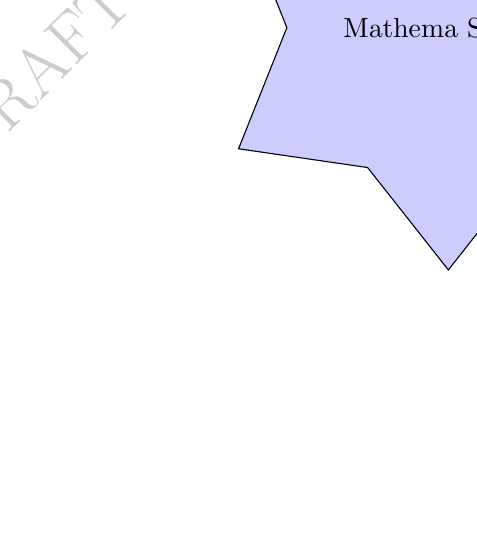
\begin{tikzpicture}
		\tikz \node [fill=blue!20,star,star points=6,draw] {Mathema Shukur };
	\end{tikzpicture}
	\\
	যাদের জন্যে প্রযোজ্যঃ  	\textcolor{magenta}{একাদশ ও দ্বাদশ শ্রেণীর শিক্ষার্থী} \\
	বিষয়ঃ \textcolor{magenta}{উচ্চতর গণিত ১ম পত্র} \\
	অধ্যায়ঃ \textcolor{magenta}{৩-সরলরেখা}\\ 
	Subtopicঃ  \textcolor{magenta}{ দুইটি সমান্তরাল সরলরেখার মধ্যবর্তী লম্ব দূরত্ব নির্ণয়  }\\
	\\
	\textcolor{blue}{$ax+by+c_1=0$ এবং $ax+by+c_2=0$ সমান্তরাল সরলরেখা দুইটির মধ্যবর্তী লম্ব দূরত্ব $d=\frac{|c_1-c_2|}{\sqrt{a^2+b^2}}$}\\
	\\
		ঢাকা  বোর্ড-২০২১\\ 
	$x+2y=2$ এবং $2x+4y=-8$ রেখাদ্বয়ের মধ্যবর্তী দূরত্ব নির্ণয় কর \\
	\begin{multicols}{2}
		\begin{align*}
		x+2y&=2\\
		\\
		x+2y-2&=0
	\end{align*}
	\\
	\begin{align*}
		2x+4y&=-8\\
		\\
		x+2y&=-4\\
		\\
		x+2y+4&=0
	\end{align*}
\begin{align*}
	a=1,\quad b=2,&\quad c_1=-2,\quad c_2=4
\end{align*}
	\end{multicols}
\begin{align*}
d&=\frac{|c_1-c_2|}{\sqrt{a^2+b^2}}\\
\\
d&=\frac{|-2-4|}{\sqrt{(1)^2+(2)^2}}=\frac{6}{\sqrt{5}}\\
\end{align*}
\\
	\\
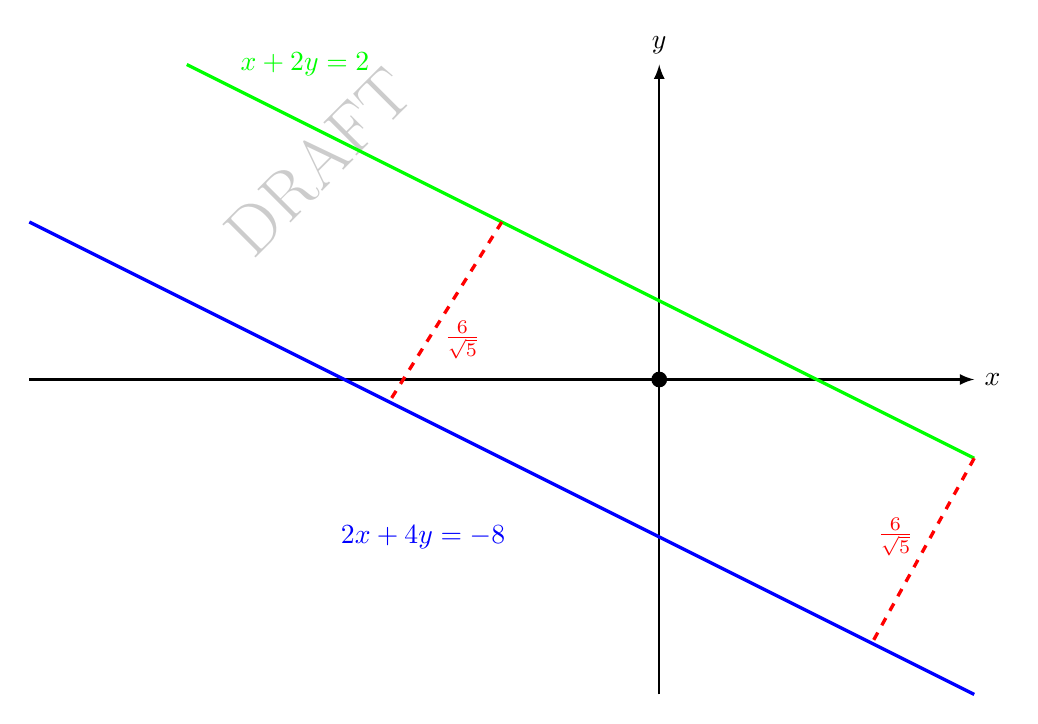
\begin{tikzpicture}[transform shape,scale=1]
	\draw [-latex,thick](-8,0) -- (4,0) node[right] {$x$} coordinate(x axis);
	\draw [-latex,thick](0,-4) -- (0,4) node[above] {$y$} coordinate(y axis);
	\fill[black] (0,0) circle (1 mm);
	\node at (-4.5,4) {$\textcolor{green}{x+2y=2}$};	
	\node at (-2.5,0.5) {$\textcolor{red}{\frac{6}{\sqrt{5}}}$};	
		\node at (3,-2) {$\textcolor{red}{\frac{6}{\sqrt{5}}}$};	
	\node at (-3,-2) {$\textcolor{blue}{2x+4y=-8}$};	
	\draw[very thick,green] (4,-1)--(-6,4);	
	\draw[very thick,blue] (-8,2)--(4,-4);	
	\draw[very thick,red,dashed] (-2,2)--(-3.43,-0.285);	
		\draw[very thick,red,dashed] (4,-1)--(2.7,-3.35);	
\end{tikzpicture}
\\
	রাজশাহী  বোর্ড-২০২১\\ 
 $4x-3y+8=0$ এবং $8x-6y+4=0$ রেখাদ্বয়ের মধ্যবর্তী লম্ব দূরত্ব নির্ণয় কর \\
	\\
	\begin{multicols}{2}
		\begin{align*}
			4x-3y+8&=0\\
		\end{align*}
		\\
		\begin{align*}
			8x-6y+4&=0\\
			\\
			4x-3y+2&=0\\
		\end{align*}
		\begin{align*}
			a=4,\quad b=-3,&\quad c_1=8,\quad c_2=2
		\end{align*}
	\end{multicols}
	\begin{align*}
		d&=\frac{|c_1-c_2|}{\sqrt{a^2+b^2}}\\
		\\
		d&=\frac{|8-2|}{\sqrt{(4)^2+(-3)^2}}\\
		\\
		d&=\frac{6}{5}\\
	\end{align*}
	\\
	\\
	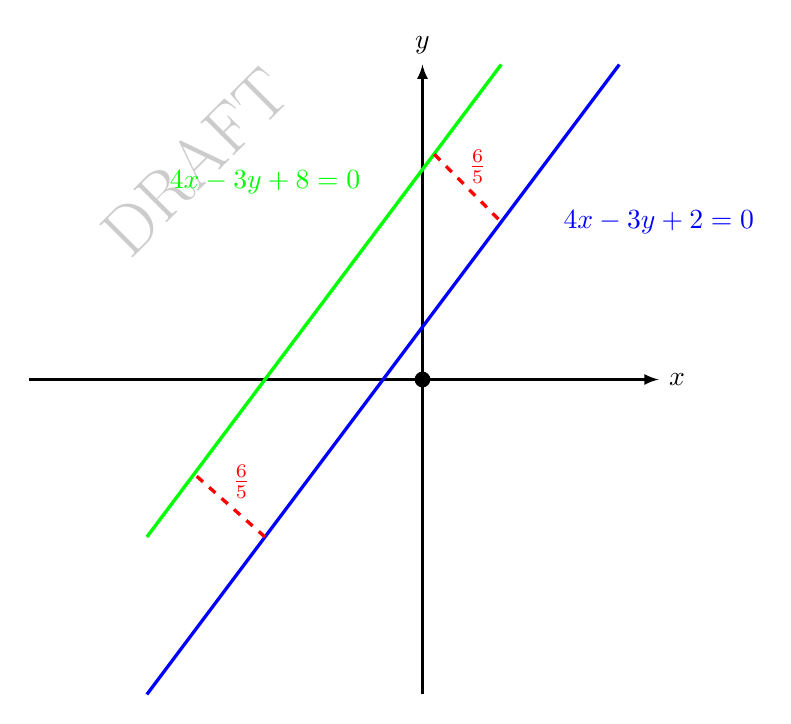
\begin{tikzpicture}[transform shape,scale=1]
		\draw [-latex,thick](-5,0) -- (3,0) node[right] {$x$} coordinate(x axis);
		\draw [-latex,thick](0,-4) -- (0,4) node[above] {$y$} coordinate(y axis);
		\fill[black] (0,0) circle (1 mm);
		\node at (-2,2.5) {$\textcolor{green}{4x-3y+8=0}$};	
		\node at (0.7,2.7) {$\textcolor{red}{\frac{6}{5}}$};	
			\node at (-2.3,-1.3) {$\textcolor{red}{\frac{6}{5}}$};	
		\node at (3,2) {$\textcolor{blue}{4x-3y+2=0}$};	
		\draw[very thick,green] (-3.5,-2)--(1,4);	
		\draw[very thick,blue] (-3.5,-4)--(2.5,4);	
		\draw[very thick,red,dashed] (0.15,2.86)--(1,2);	
			\draw[very thick,red,dashed] (-2,-2)--(-2.9,-1.2);	
	\end{tikzpicture}
\end{document}